La clase anterior terminó mostrando que $\pi_{k+1}(\Sigma X)\cong\pi_k(X)$ y, por otra parte y de manera más directa, que $\pi_k(X)\cong\pi_{k+1}(sh^1X)$. Los dos espectros $\Sigma X$ y $sh^1X$ tienen por tanto los mismos grupos de homotopía, lo que los hace buenos candidatos a ser establemente equivalentes, pero el cálculo de los grupos no basta: hace falta exhibir un morfismo, o un zigzag de morfismos, que realice el isomorfismo. Esta clase construye ese zigzag, y con él queda demostrado que la suspensión es invertible en la categoría homotópica estable.

El camino tiene tres etapas. Primero se introduce la noción de \emph{morfismo débil}, que relaja la condición de conmutatividad de los morfismos de espectros admitiendo homotopías, y se muestra que todo morfismo débil se puede reemplazar por un zigzag en el que uno de los morfismos es una equivalencia nivel a nivel. Después se construye, para cada espectro $X$, un espectro ``par'' que conserva la información de los niveles pares y descarta la de los impares, y se prueba que es establemente equivalente a $X$. Finalmente se combinan ambas herramientas para conectar $\Sigma X$ con $sh^1X$. La última parte de la clase, más ligera, recoge una serie de construcciones con espectros ---el producto smash con un espacio, el espectro de funciones, los (co)límites y las (co)fibras--- que se usarán más adelante.

% A lo largo del capítulo los morfismos estructurales de un espectro se escriben $\xi_n\colon\Sigma X_n\to X_{n+1}$, como en los capítulos anteriores. Cuando intervienen dos espectros a la vez, los del segundo se escriben $\xi'_n$, y los del espectro par de la \myref{defi:espectro-par} se escriben $\xi^{\mathrm{par}}_n$ para no confundirlos con los de $X$.

%%%%%%%%%%%%%%%%%%%%%%%%%%%%%%%%%%%%%%%%%%%%%%%%%%%%%%%%%%%%%%%%%%%%%%%%%%%%%%%
\section{Morfismos débiles y el telescopio}
%%%%%%%%%%%%%%%%%%%%%%%%%%%%%%%%%%%%%%%%%%%%%%%%%%%%%%%%%%%%%%%%%%%%%%%%%%%%%%%

La primera herramienta es una noción relajada de morfismo de espectros. La motivación es la siguiente: en la demostración del isomorfismo $\pi_{k+1}(\Sigma X)\cong\pi_k(X)$ lo que aparecía no era un cuadrado conmutativo, sino un cuadrado que conmutaba \emph{salvo} una permutación de esferas, y esa permutación tenía un signo que solo se corregía al recorrer dos niveles de golpe. Un morfismo débil es exactamente lo que hay que admitir para trabajar con esa situación.

%%%%%%%%%%%%%%%%%%%%%%%%%%%%%%%%%%%%%%%%%%%%%%%%%%%%%%%%%%%%%%%%%%%%%%%%%%%%%%%
\subsection{Morfismos débiles}
%%%%%%%%%%%%%%%%%%%%%%%%%%%%%%%%%%%%%%%%%%%%%%%%%%%%%%%%%%%%%%%%%%%%%%%%%%%%%%%

\begin{defi}\label{defi:morfismo-debil}
Sean $A$ y $B$ espectros secuenciales. Un \emph{morfismo débil} de $A$ a $B$ consiste en aplicaciones punteadas $f_n\colon A_n\to B_n$ y homotopías punteadas
\[
H_n\colon\Sigma A_n\wedge I_+\longrightarrow B_{n+1}
\]
tales que el siguiente diagrama conmuta salvo la homotopía $H_n$:
\[
\begin{tikzcd}[column sep=huge, row sep=large]
\Sigma A_n \arrow[r,"\Sigma f_n"] \arrow[d,"\xi_n"'] & \Sigma B_n \arrow[d,"\xi'_n"]\\
A_{n+1} \arrow[r,"f_{n+1}"'] \arrow[ur,Rightarrow,"H_n",nfold] & B_{n+1}
\end{tikzcd}
\]
Es decir, $H_n$ es una homotopía de $f_{n+1}\circ\xi_n$ a $\xi'_n\circ\Sigma f_n$, donde $\xi_*$ y $\xi'_*$ son los morfismos estructurales de $A$ y de $B$.
\end{defi}

Un morfismo de espectros es, en particular, un morfismo débil: basta tomar $H_n$ constante. Lo que se gana al relajar la condición es que los morfismos débiles son mucho más fáciles de construir, y lo que se pierde ---no poder componerlos de la manera obvia--- se recupera con la construcción de la subsección siguiente.

%%%%%%%%%%%%%%%%%%%%%%%%%%%%%%%%%%%%%%%%%%%%%%%%%%%%%%%%%%%%%%%%%%%%%%%%%%%%%%%
\subsection{El telescopio asociado a un morfismo débil}
%%%%%%%%%%%%%%%%%%%%%%%%%%%%%%%%%%%%%%%%%%%%%%%%%%%%%%%%%%%%%%%%%%%%%%%%%%%%%%%

Sea $(f_*,H_*)\colon A\to B$ un morfismo débil. La idea es reemplazar $A$ por un espectro equivalente sobre el que las homotopías se hayan vuelto conmutatividades estrictas. Ese reemplazo es el \emph{telescopio} o \emph{colímite homotópico secuencial}.

\begin{defi}\label{defi:telescopio}
Se define, para cada $n\ge0$,
\[
C_n\coloneqq A_n\cup_{\xi_{n-1}}\bigl(\Sigma A_{n-1}\wedge I_+\bigr)\cup_{\Sigma\xi_{n-2}}\bigl(\Sigma^2A_{n-2}\wedge I_+\bigr)\cup_{\Sigma^{2}\xi_{n-3}}\cdots\cup_{\Sigma^{n-1}\xi_0}\bigl(\Sigma^{n-1}A_0\wedge I_+\bigr),
\]
donde los $\Sigma^{k}A_{n-k}\wedge I_+$ se pegan por sus bases mediante $\Sigma^{k}\xi_{n-1-k}$.
\end{defi}

Geométricamente, $C_{n}$ se construye empezando con $A_{n}$ y pegando sucesivamente \enquote{cilindros} con base $\Sigma^k A_{n-k}$ mediante los mapas $\Sigma^{k}\xi_{n-1-k}$. La siguiente figura lo esquematiza.

\begin{center}
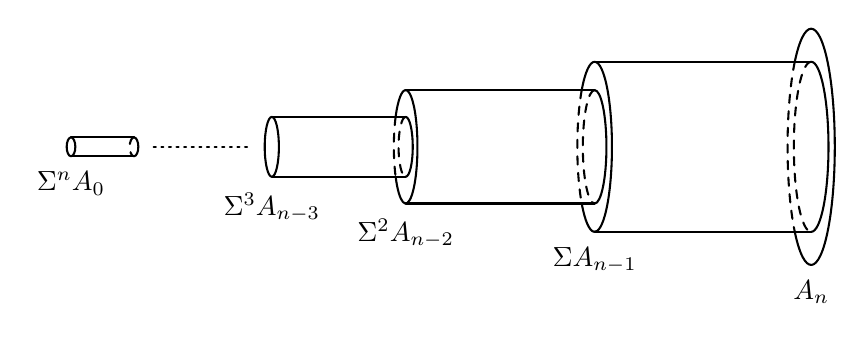
\begin{tikzpicture}[x=1cm,y=1cm,line width=.75pt,
                    line cap=round,line join=round]
  % Las dos primeras tapas izquierdas son completamente visibles.
  \def\tapaVisible#1#2#3{%
    \draw (#1,0) ellipse [x radius=#2,y radius=#3];%
  }
  % Tapa derecha: su mitad izquierda queda oculta.
  \def\tapaDerecha#1#2#3{%
    \draw[dashed] (#1,#3)
      arc[start angle=90,end angle=270,x radius=#2,y radius=#3];
    \draw (#1,#3)
      arc[start angle=90,end angle=-90,x radius=#2,y radius=#3];%
  }
  % Tapa izquierda: solo se oculta el arco comprendido entre
  % las paredes y=+#4 e y=-#4 del cilindro anterior.
  \def\tapaIzquierda#1#2#3#4{%
    \pgfmathsetmacro{\anguloOculto}{asin(#4/#3)}%
    \draw (#1,#3)
      arc[start angle=90,end angle={180-\anguloOculto},
          x radius=#2,y radius=#3];
    \draw[dashed] ({#1-#2*cos(\anguloOculto)},{#4})
      arc[start angle={180-\anguloOculto},end angle={180+\anguloOculto},
          x radius=#2,y radius=#3];
    \draw ({#1-#2*cos(\anguloOculto)},{-#4})
      arc[start angle={180+\anguloOculto},end angle=450,
          x radius=#2,y radius=#3];%
  }

  \draw (0,.12) -- (.80,.12) (0,-.12) -- (.80,-.12);
  \tapaVisible{0}{.055}{.12}
  \tapaDerecha{.80}{.055}{.12}
  \node[below=2pt] at (0,-.12) {$\Sigma^{n}A_0$};
  \draw[dotted] (1.05,0) -- (2.30,0);

  \draw (2.55,.38) -- (4.25,.38)
        (2.55,-.38) -- (4.25,-.38);
  \tapaVisible{2.55}{.09}{.38}
  \tapaDerecha{4.25}{.09}{.38}
  \node[below=2pt] at (2.55,-.38) {$\Sigma^3A_{n-3}$};

  \draw (4.25,.72) -- (6.65,.72)
        (4.25,-.72) -- (6.65,-.72);
  \tapaIzquierda{4.25}{.15}{.72}{.38}
  \tapaDerecha{6.65}{.15}{.72}
  \node[below=2pt] at (4.25,-.72) {$\Sigma^2A_{n-2}$};

  \draw (6.65,1.08) -- (9.40,1.08)
        (6.65,-1.08) -- (9.40,-1.08);
  \tapaIzquierda{6.65}{.22}{1.08}{.72}
  \tapaDerecha{9.40}{.22}{1.08}
  \node[below=2pt] at (6.65,-1.08) {$\Sigma A_{n-1}$};

  \tapaIzquierda{9.40}{.30}{1.50}{1.08}
  \node[below=2pt] at (9.40,-1.50) {$A_{n}$};
\end{tikzpicture}
\end{center}

\begin{prop}\label{prop:nu-bien-definido}
La asignación
\[
\nu_n\colon\Sigma C_n\longrightarrow C_{n+1},
\qquad
[x,s,t,u]\longmapsto[x,s,u,t],
\]
donde $x\in A_k$, $s$ recoge las coordenadas de suspensión en $\Sigma^{n-k}A_k$, $t$ es la coordenada en $I_+$ del cilindro y $u$ es la coordenada de la última suspensión, está bien definida y dota a $C=(C_n,\nu_n)$ de estructura de espectro secuencial.
\end{prop}

\begin{proof}
El punto delicado es la compatibilidad con las identificaciones del telescopio. En $\Sigma C_n$ los elementos $[x,s,0,u]$ y $[\Sigma^{n-k-1}\xi_k(x,s),1,u]$ representan la misma clase, porque $[x,s,0]$ es la base superior del cilindro $\Sigma^{n-k}A_k\wedge I_+$ y $[\Sigma^{n-k-1}\xi_k(x,s),1]$ es la base inferior del cilindro siguiente. Aplicando $\nu_n$ a ambos se obtiene
\[
[x,s,u,0]
\qquad\text{y}\qquad
[\Sigma^{n-k-1}\xi_k(x,s),u,1],
\]
y hay que comprobar que estas dos clases coinciden en $C_{n+1}$. En efecto, en $C_{n+1}$ la identificación que define el telescopio es precisamente
\[
[\Sigma^{n-k-1}\xi_k(x,s),u,1]=[x,s,u,0],
\]
pues la coordenada $u$ no interviene en la relación de pegadura y puede atravesarla. Por tanto $\nu_n$ está bien definida. La comprobación de que $\nu$ es compatible con las estructuras, es decir, que dota a $C$ de estructura de espectro, es la misma cuenta aplicada a cada nivel. \qedhere
\end{proof}

%%%%%%%%%%%%%%%%%%%%%%%%%%%%%%%%%%%%%%%%%%%%%%%%%%%%%%%%%%%%%%%%%%%%%%%%%%%%%%%
\subsection{El morfismo que aplasta el telescopio}
%%%%%%%%%%%%%%%%%%%%%%%%%%%%%%%%%%%%%%%%%%%%%%%%%%%%%%%%%%%%%%%%%%%%%%%%%%%%%%%

\begin{prop}\label{prop:p-espectro}
Las equivalencias homotópicas
\[
p_n\colon C_n\longrightarrow A_n
\]
que aplastan todos los cilindros del telescopio sobre $A_n$ conforman un morfismo de espectros $p\colon C\to A$. Es decir, $p$ es una equivalencia nivel a nivel.
\end{prop}

\begin{proof}
Probemos que $p$ conmuta con los morfismos estructurales, es decir, que el cuadrado
\[
\begin{tikzcd}[column sep=huge, row sep=large]
\Sigma C_n \arrow[r,"\nu_n"] \arrow[d,"\Sigma p_n"'] & C_{n+1} \arrow[d,"p_{n+1}"]\\
\Sigma A_n \arrow[r,"\xi_n"'] & A_{n+1}
\end{tikzcd}
\]
conmuta. Tomando un elemento $[x,s,t,u]$ con $x\in A_k$,
\[
\Sigma p_n[x,s,t,u]=\bigl[\xi_{n-1}\circ\cdots\circ\Sigma^{n-k-1}\xi_k(x,s),\,u\bigr],
\;\;\implies\;\;
\xi_n\bigl(\Sigma p_n[x,s,t,u]\bigr)=\xi_n\circ\Sigma\xi_{n-1}\circ\cdots\circ\Sigma^{n-k}\xi_k(x,s,u)
\]
Asimismo,
\[
\xi_{n-1}\circ\Sigma\xi_{n-2}\circ\cdots\circ\Sigma^{n-k}\xi_k(x,s,u).
\]
Las dos expresiones coinciden porque, al incorporar $u$ como coordenada nueva, lo que se está haciendo es introducir una suspensión adicional, y suspender y aplicar el morfismo estructural conmutan por definición de $\nu$. \qedhere
\end{proof}

%%%%%%%%%%%%%%%%%%%%%%%%%%%%%%%%%%%%%%%%%%%%%%%%%%%%%%%%%%%%%%%%%%%%%%%%%%%%%%%
\subsection{El morfismo hacia el segundo espectro}
%%%%%%%%%%%%%%%%%%%%%%%%%%%%%%%%%%%%%%%%%%%%%%%%%%%%%%%%%%%%%%%%%%%%%%%%%%%%%%%

El segundo morfismo que sale del telescopio es el que usa las homotopías del morfismo débil.

\begin{prop}\label{prop:fprima-espectro}
Sea $(f_*,H_*)\colon A\to B$ un morfismo débil. Entonces existe un morfismo de espectros
\[
f'_n\colon C_n\longrightarrow B_n
\]
definido por casos según en qué cilindro del telescopio esté el elemento:
\[
f'_n\bigl([x]\bigr)=f_n(x)\quad\text{si }x\in A_n,
\]
\[
f'_n\bigl([x,s_1,t]\bigr)=H_{n-1}\bigl([x,s_1,t]\bigr)\quad\text{si }x\in A_{n-1},
\]
\[
f'_n\bigl([x,s_1,s_2,t]\bigr)=\xi'_{n-1}\circ\Sigma H_{n-2}\bigl([x,s_1,s_2,t]\bigr)\quad\text{si }x\in A_{n-2},
\]
y en general, para $x\in A_{n-k}$,
\[
f'_n\bigl([x,s,t]\bigr)=\xi'_{n-1}\circ\Sigma\xi'_{n-2}\circ\cdots\circ\Sigma^{k-2}\xi'_{n-k+1}\circ\Sigma^{k-1}H_{n-k}\bigl([x,s,t]\bigr).
\]
\end{prop}

\begin{proof}
La fórmula tiene la siguiente lectura: la homotopía $H_{n-k}$ sólo ``come'' elementos de $\Sigma A_{n-k}\wedge I_+$ y devuelve elementos de $B_{n-k+1}$, de modo que hay que suspenderla $k-1$ veces para que su imagen viva en $B_n$, y a continuación aplicar los morfismos estructurales $\xi'$ de $B$ las veces necesarias. La comprobación de que $f'_n$ está bien definida es la parte delicada, y consiste en verificar que los dos representantes de una misma clase del telescopio reciben la misma imagen.

Sean $[x,s,0]$ y $[\Sigma^{n-k-1}\xi_k(x,s),1]$ los dos representantes de un punto de pegadura. Por una parte, aplicando la fórmula al primero y usando que la homotopía $H_{n-k}$ evaluada en $t=0$ es $f_{n-k+1}\circ\xi_{n-k}$, se obtiene
\[
\xi'_{n-1}\circ\Sigma\xi'_{n-2}\circ\cdots\circ\Sigma^{n-k-2}\xi'_{k+1}\circ\Sigma^{n-k-1}f_{k+1}\circ\Sigma^{n-k-1}\xi_k(x,s).
\]
Por otra parte, aplicando la fórmula al segundo, y usando que $H_{n-k}$ evaluada en $t=1$ es $\xi'_{n-k}\circ\Sigma f_{n-k}$, se obtiene
\[
\xi'_{n-1}\circ\Sigma\xi'_{n-2}\circ\cdots\circ\Sigma^{n-k-2}\xi'_{k+1}\circ\Sigma^{n-k-1}\xi'_k\circ\Sigma^{n-k-1}\xi_k(x,s).
\]
Las dos expresiones coinciden porque $f$ es un morfismo, es decir, porque el cuadrado de la \myref{defi:espectro-secuencial} conmuta, de modo que
\[
\Sigma^{n-k-1}f_{k+1}\circ\Sigma^{n-k-1}\xi_k=\Sigma^{n-k-1}\xi'_k\circ\Sigma^{n-k-1}f_k,
\]
y el término $\Sigma^{n-k-1}f_k$ puede reabsorberse en la homotopía del paso anterior, que es precisamente lo que garantiza la compatibilidad de las suspensiones de las homotopías. La verificación de que $f'$ conmuta con los morfismos estructurales, es decir, que el cuadrado
\[
\begin{tikzcd}[column sep=huge, row sep=large]
\Sigma C_n \arrow[r,"\Sigma f'_n"] \arrow[d,"\nu_n"'] & \Sigma B_n \arrow[d,"\xi'_n"]\\
C_{n+1} \arrow[r,"f'_{n+1}"'] & B_{n+1}
\end{tikzcd}
\]
conmuta \emph{estrictamente} ---no solo salvo homotopía---, es una cuenta análoga sobre las coordenadas, en la que el único punto que hay que observar es que la coordenada $u$ que introduce $\nu$ puede atravesar todos los morfismos estructurales, lo que vuelve a ser la observación de que suspender y aplicar el morfismo estructural conmutan. \qedhere
\end{proof}

\begin{nota}
   El profesor hizo hincapié en que estas cuentas, aunque pesadas, tienen un valor que no se ve hasta hacerlas: en homotopía estable hay muchos diagramas que hay que comprobar y muchos signos que provienen de permutar esferas, y la razón de ser de esos signos no se entiende hasta que uno localiza exactamente dónde falla la conmutatividad. La observación es la misma que motivó el paso a los índices pares en el cálculo de $\pi_{k+1}(\Sigma X)$.
\end{nota}

Con los dos morfismos construidos se tiene el zigzag que reemplaza al morfismo débil.

\begin{teo}\label{teo:zigzag-morfismo-debil}
Sea $(f_*,H_*)\colon A\to B$ un morfismo débil. Entonces el zigzag
\[
A\xleftarrow{\ p\ }C\xrightarrow{\ f'\ }B
\]
define un morfismo de $A$ a $B$ en la categoría $\Sp_N[\text{equiv.\ estables}^{-1}]$, es decir, en la categoría homotópica estable. Además el diagrama
\[
\begin{tikzcd}[column sep=huge, row sep=large]
C_n \arrow[r,"f'_n"] \arrow[d,"p_n"'] & B_n\\
A_n \arrow[ru,"f_n"'] &
\end{tikzcd}
\]
conmuta salvo homotopía.
\end{teo}

\begin{proof}
La primera afirmación es consecuencia de la \myref{prop:p-espectro}: como $p$ es una equivalencia nivel a nivel, y en particular una equivalencia estable, se puede invertir formalmente en la categoría localizada, y el zigzag define un morfismo de $A$ a $B$.

Para la conmutatividad salvo homotopía, sea $i_n\colon A_n\to C_n$ la inclusión del nivel $A_n$ en el telescopio. Por construcción de $f'$, sobre $A_n$ la fórmula es simplemente $f'_n\circ i_n=f_n$, es decir, $f'_n i_n=f_n$ como aplicaciones. Por otra parte $i_n\circ p_n$ no es la identidad, porque un elemento de $C_n$ puede estar en un cilindro y no en $A_n$, pero sí es homótopo a la identidad: aplastar un cilindro y volver a incluirlo es homótopo a no hacer nada, ya que cada cilindro es contráctil. Componiendo la igualdad $f'_ni_n=f_n$ con $p_n$ por la derecha se obtiene
\[
f'_n i_n p_n=f_n p_n,
\]
y como $i_np_n\simeq\id$, resulta $f'_n\simeq f_n$. \qedhere
\end{proof}

\begin{coro}\label{coro:debil-equivalencia}
Si en un morfismo débil todas las aplicaciones $f_n$ son equivalencias homotópicas, entonces el morfismo $f'$ del \myref{teo:zigzag-morfismo-debil} es una equivalencia nivel a nivel y, por tanto, una equivalencia estable.
\end{coro}

\begin{proof}
Por el \myref{teo:zigzag-morfismo-debil} se tiene $f'_n\simeq f_n$ para todo $n$, de modo que $f'_n$ es una equivalencia homotópica siempre que lo sea $f_n$. Como esto ocurre en todos los niveles, $f'$ es una equivalencia nivel a nivel. \qedhere
\end{proof}

%%%%%%%%%%%%%%%%%%%%%%%%%%%%%%%%%%%%%%%%%%%%%%%%%%%%%%%%%%%%%%%%%%%%%%%%%%%%%%%
\section{El espectro par}
%%%%%%%%%%%%%%%%%%%%%%%%%%%%%%%%%%%%%%%%%%%%%%%%%%%%%%%%%%%%%%%%%%%%%%%%%%%%%%%

La segunda herramienta es una construcción que permite ``quedarse con los niveles pares'' de un espectro. El obstáculo es evidente: un espectro secuencial tiene niveles en \emph{todos} los grados, de modo que no se puede simplemente descartar los impares. Lo que se hace es conservar los niveles pares y rellenar los impares con lo mínimo necesario para que el espectro siga existiendo y para que los niveles pares queden conectados entre sí.

%%%%%%%%%%%%%%%%%%%%%%%%%%%%%%%%%%%%%%%%%%%%%%%%%%%%%%%%%%%%%%%%%%%%%%%%%%%%%%%
\subsection{La construcción del espectro par}
%%%%%%%%%%%%%%%%%%%%%%%%%%%%%%%%%%%%%%%%%%%%%%%%%%%%%%%%%%%%%%%%%%%%%%%%%%%%%%%

\begin{defi}\label{defi:espectro-par}
Sea $X$ un espectro secuencial. Su \emph{espectro par} $X^{\mathrm{par}}$ es el espectro secuencial cuyos niveles son
\[
X^{\mathrm{par}}_{2n}\coloneqq X_{2n},
\qquad
X^{\mathrm{par}}_{2n+1}\coloneqq X_{2n}\wedge S^1,
\]
y cuyos morfismos estructurales son
\[
\xi^{\mathrm{par}}_{2n}\colon X_{2n}\wedge S^1\xrightarrow{\ 1\ }X_{2n}\wedge S^1 ,
\qquad
\xi^{\mathrm{par}}_{2n+1}\colon X_{2n}\wedge S^1\wedge S^1\longrightarrow X_{2n+2},
\]
donde el segundo se define como la composición
\[
X_{2n}\wedge S^1\wedge S^1\xrightarrow{\ \xi_{2n}\wedge1\ }X_{2n+1}\wedge S^1\xrightarrow{\ \xi_{2n+1}\ }X_{2n+2}.
\]
\end{defi}

Es decir: del nivel impar $X_{2n+1}$ del espectro original no se conserva nada; en su lugar se pone $X_{2n}\wedge S^1$, que es el nivel par anterior con una esfera adjuntada. El morfismo estructural del nivel par al impar es la identidad, y el del impar al par siguiente usa los dos morfismos estructurales originales. En la pizarra este espectro se escribió $X^{even}$, con el rótulo inglés.

En la pizarra la construcción se ilustró con una tabla que compara los niveles de tres espectros: el original $X$, su desplazamiento $sh^1X$ y el espectro par de ese desplazamiento. Conviene tenerla a la vista porque es la que explica por qué la construcción funciona.

\begin{center}
\begin{tabular}{c|c|c|c}
 & $sh^1X$ & $X^{\mathrm{par}}$ & $\bigl(sh^1X\bigr)^{\mathrm{par}}$\\\hline
$0$ & $X_1$ & $X_0\wedge S^1$ & $X_0\wedge S^1$\\
$1$ & $X_2$ & $X_2$ & $(X_0\wedge S^1)\wedge S^1$\\
$2$ & $X_3$ & $X_2\wedge S^1$ & $X_2\wedge S^1$
\end{tabular}
\end{center}

Los morfismos estructurales de la tercera columna son $\xi'_1\circ\Sigma\xi'_0$ del par al impar, la identidad al revés, y $(\xi_1\circ\Sigma\xi_0)\wedge1$ en el último salto.

%%%%%%%%%%%%%%%%%%%%%%%%%%%%%%%%%%%%%%%%%%%%%%%%%%%%%%%%%%%%%%%%%%%%%%%%%%%%%%%
\subsection{El morfismo hacia el espectro original}
%%%%%%%%%%%%%%%%%%%%%%%%%%%%%%%%%%%%%%%%%%%%%%%%%%%%%%%%%%%%%%%%%%%%%%%%%%%%%%%

\begin{prop}\label{prop:g-morfismo}
Sea $X$ un espectro secuencial. La asignación
\[
g_{2n}\colon X^{\mathrm{par}}_{2n}\xrightarrow{\ 1\ }X_{2n},
\qquad
g_{2n+1}\colon X^{\mathrm{par}}_{2n+1}=X_{2n}\wedge S^1\xrightarrow{\ \xi_{2n}\ }X_{2n+1},
\]
define un morfismo de espectros $g\colon X^{\mathrm{par}}\to X$.
\end{prop}

\begin{proof}
Hay que comprobar dos tipos de cuadrados, según la paridad del nivel de partida. Para el paso de un nivel par a un nivel impar, el cuadrado es
\[
\begin{tikzcd}[column sep=huge, row sep=large]
\Sigma X^{\mathrm{par}}_{2n} \arrow[r,"\Sigma g_{2n}"] \arrow[d,"\xi^{\mathrm{par}}_{2n}"'] & \Sigma X_{2n} \arrow[d,"\xi_{2n}"]\\
X^{\mathrm{par}}_{2n+1} \arrow[r,"g_{2n+1}"'] & X_{2n+1}
\end{tikzcd}
\]
y conmuta porque $\xi^{\mathrm{par}}_{2n}$ es la identidad y $g_{2n+1}$ es precisamente $\xi_{2n}$, mientras que $g_{2n}$ es la identidad. Para el paso de un nivel impar a un nivel par, el cuadrado es
\[
\begin{tikzcd}[column sep=huge, row sep=large]
\Sigma X^{\mathrm{par}}_{2n+1} \arrow[r,"\Sigma g_{2n+1}"] \arrow[d,"\xi^{\mathrm{par}}_{2n+1}"'] & \Sigma X_{2n+1} \arrow[d,"\xi_{2n+1}"]\\
X^{\mathrm{par}}_{2n+2} \arrow[r,"g_{2n+2}"'] & X_{2n+2}
\end{tikzcd}
\]
y conmuta porque $\xi^{\mathrm{par}}_{2n+1}$ es la composición $\xi_{2n+1}\circ(\xi_{2n}\wedge1)$, que es exactamente lo que resulta de suspender $g_{2n+1}=\xi_{2n}$ y componer con $\xi_{2n+1}$, mientras que $g_{2n+2}$ es la identidad. En ambos casos la conmutatividad es estricta. \qedhere
\end{proof}

%%%%%%%%%%%%%%%%%%%%%%%%%%%%%%%%%%%%%%%%%%%%%%%%%%%%%%%%%%%%%%%%%%%%%%%%%%%%%%%
\subsection{El espectro par es establemente equivalente al original}
%%%%%%%%%%%%%%%%%%%%%%%%%%%%%%%%%%%%%%%%%%%%%%%%%%%%%%%%%%%%%%%%%%%%%%%%%%%%%%%

\begin{teo}\label{teo:par-equivalente}
Para todo espectro secuencial $X$, el morfismo $g\colon X^{\mathrm{par}}\to X$ de la \myref{prop:g-morfismo} es una equivalencia estable.
\end{teo}

\begin{proof}
Hay que ver que $g_*\colon\pi_k(X^{\mathrm{par}})\to\pi_k(X)$ es un isomorfismo para todo $k$. Los dos grupos son colímites,
\[
\pi_k\bigl(X^{\mathrm{par}}\bigr)=\varinjlim_m\pi_{m+k}\bigl(X^{\mathrm{par}}_m\bigr),
\qquad
\pi_k(X)=\varinjlim_m\pi_{m+k}(X_m),
\]
y el sistema de índices admite el subconjunto cofinal de los índices pares $m=2m'$. Restringiendo ambos sistemas a esos índices se obtiene el diagrama
\[
\begin{tikzcd}[column sep=huge, row sep=large]
\pi_k\bigl(X^{\mathrm{par}}\bigr) \arrow[d,"\cong"'] & \varinjlim_m\pi_{m+k}\bigl(X^{\mathrm{par}}_m\bigr) \arrow[l,"\cong"'] \arrow[d,"\varinjlim_m (g_m)_*"] & \varinjlim_m\pi_{2m+k}\bigl(X^{\mathrm{par}}_{2m}\bigr) \arrow[l,"\cong"'] \arrow[d,"\varinjlim_m (g_{2m})_*"]\\
\pi_k(X) & \varinjlim_m\pi_{m+k}(X_m) \arrow[l,"\cong"'] & \varinjlim_m\pi_{2m+k}(X_{2m}) \arrow[l,"\cong"']
\end{tikzcd}
\]
en el que las flechas horizontales son isomorfismos por cofinalidad. En la columna derecha, $X^{\mathrm{par}}_{2m}=X_{2m}$ y $g_{2m}$ es la identidad, de modo que $\varinjlim_m(g_{2m})_*$ es la identidad y por tanto un isomorfismo. Como el diagrama conmuta y las otras tres flechas son isomorfismos, $g_*$ es un isomorfismo. \qedhere
\end{proof}

\begin{nota}
   El argumento se apoya en un hecho que conviene aislar: los grupos de homotopía de un espectro están definidos como un colímite sobre un sistema dirigente, y eso permite reemplazar el sistema por cualquier subsistema cofinal sin alterar el resultado. Aquí el subsistema es el de los índices pares. El profesor señaló que la misma construcción funciona con los múltiplos de cualquier entero positivo: basta rellenar los huecos con productos smash sucesivos con $S^1$, y el espectro resultante sigue siendo establemente equivalente al original. En la práctica solo se usa el caso par, porque es el que realiza a nivel de espectros el paso a los índices pares que apareció en el cálculo de $\pi_{k+1}(\Sigma X)$.
\end{nota}

%%%%%%%%%%%%%%%%%%%%%%%%%%%%%%%%%%%%%%%%%%%%%%%%%%%%%%%%%%%%%%%%%%%%%%%%%%%%%%%
\section{La estabilidad de la categoría homotópica estable}
%%%%%%%%%%%%%%%%%%%%%%%%%%%%%%%%%%%%%%%%%%%%%%%%%%%%%%%%%%%%%%%%%%%%%%%%%%%%%%%

Con las dos herramientas anteriores se puede ya demostrar el resultado que da nombre a la sección.

%%%%%%%%%%%%%%%%%%%%%%%%%%%%%%%%%%%%%%%%%%%%%%%%%%%%%%%%%%%%%%%%%%%%%%%%%%%%%%%
\subsection{La cadena de equivalencias}
%%%%%%%%%%%%%%%%%%%%%%%%%%%%%%%%%%%%%%%%%%%%%%%%%%%%%%%%%%%%%%%%%%%%%%%%%%%%%%%

El primer paso es aplicar la construcción del espectro par a los dos espectros que se quieren comparar. Como $X^{\mathrm{par}}$ es establemente equivalente a $X$, y el desplazamiento y la suspensión son funtores, se obtienen equivalencias estables
\[
\Sigma X\xleftarrow{\ \simeq_s\ }\bigl(\Sigma X\bigr)^{\mathrm{par}},
\qquad
sh^1X\xleftarrow{\ \simeq_s\ }sh^1\bigl(X^{\mathrm{par}}\bigr),
\qquad
sh^1\bigl(X^{\mathrm{par}}\bigr)\xleftarrow{\ \simeq_s\ }sh^1\bigl(X^{\mathrm{par}}\bigr)^{\mathrm{par}} .
\]
El segundo desplazamiento se debe a que $sh^1X$ tiene niveles $X_{n+1}$, y su espectro par conserva los niveles de la forma $X_{2n}\wedge S^1$; por eso hay que tomar primero el espectro par de $X$ y después desplazarlo, y luego volver a tomar el espectro par. Las tres flechas apuntan hacia la izquierda porque la equivalencia estable va de $X^{\mathrm{par}}$ a $X$, y se han invertido para encadenarlas.

%%%%%%%%%%%%%%%%%%%%%%%%%%%%%%%%%%%%%%%%%%%%%%%%%%%%%%%%%%%%%%%%%%%%%%%%%%%%%%%
\subsection{El morfismo débil entre los espectros pares}
%%%%%%%%%%%%%%%%%%%%%%%%%%%%%%%%%%%%%%%%%%%%%%%%%%%%%%%%%%%%%%%%%%%%%%%%%%%%%%%

\begin{prop}\label{prop:debil-pares}
Las aplicaciones $f_n\colon X_{2n}\wedge S^1\to S^1\wedge X_{2n}$ que intercambian los dos factores definen un morfismo débil
\[
sh^1\bigl(X^{\mathrm{par}}\bigr)^{\mathrm{par}}\longrightarrow\bigl(\Sigma X\bigr)^{\mathrm{par}},
\]
tomando $f_n$ en el nivel $2n$ y $f_n\wedge1$ en el nivel $2n+1$. Además, en cada nivel es un homeomorfismo.
\end{prop}

\begin{proof}
Hay que comprobar los dos cuadrados, el que va de un nivel par a un nivel impar y el que va del impar al par siguiente. El primero es
\[
\begin{tikzcd}[column sep=huge, row sep=large]
X_{2n}\wedge S^1\wedge S^1 \arrow[r,"\Sigma f_n"] \arrow[d,equal] & S^1\wedge X_{2n}\wedge S^1 \arrow[d,equal]\\
X_{2n}\wedge S^1\wedge S^1 \arrow[r,"f_n\wedge1"'] & S^1\wedge X_{2n}\wedge S^1
\end{tikzcd}
\]
y conmuta \emph{estrictamente}, porque los morfismos estructurales de los dos espectros pares son la identidad en este paso y $\Sigma f_n$ es, por definición de la suspensión de una aplicación, la misma aplicación que $f_n\wedge1$ una vez identificadas las suspensiones. El segundo cuadrado es
\[
\begin{tikzcd}[column sep=huge, row sep=large]
X_{2n}\wedge S^1\wedge S^1\wedge S^1 \arrow[r,"\Sigma(f_n\wedge1)"] \arrow[d,"(\xi_{2n+1}\circ\Sigma\xi_{2n})\wedge1"'] & S^1\wedge X_{2n}\wedge S^1\wedge S^1 \arrow[d,"1\wedge(\xi_{2n+1}\circ\Sigma\xi_{2n})"]\\
X_{2n+2}\wedge S^1 \arrow[r,"f_{n+1}"'] & S^1\wedge X_{2n+2}
\end{tikzcd}
\]
y este es exactamente el diagrama que en la clase anterior no conmutaba, sino que conmutaba salvo homotopía, y cuya falta de conmutatividad era una permutación de esferas. Por tanto aquí sí hay una homotopía que lo llena, y el morfismo es un morfismo débil.

Que cada nivel sea un homeomorfismo es inmediato: $f_n$ intercambia los dos factores de un producto smash, lo que es un homeomorfismo. \qedhere
\end{proof}

%%%%%%%%%%%%%%%%%%%%%%%%%%%%%%%%%%%%%%%%%%%%%%%%%%%%%%%%%%%%%%%%%%%%%%%%%%%%%%%
\subsection{La conclusión}
%%%%%%%%%%%%%%%%%%%%%%%%%%%%%%%%%%%%%%%%%%%%%%%%%%%%%%%%%%%%%%%%%%%%%%%%%%%%%%%

\begin{teo}\label{teo:sigma-sh}
En la categoría $\Sp_N[\text{equiv.\ estables}^{-1}]$ los funtores $\Sigma$ y $sh^1$ son naturalmente isomorfos. En particular, la suspensión es invertible salvo isomorfismo natural, y la categoría homotópica estable es estable.
\end{teo}

\begin{proof}
Por la \myref{prop:debil-pares} se tiene un morfismo débil entre los espectros pares, y por el \myref{coro:debil-equivalencia}, como cada nivel es un homeomorfismo y en particular una equivalencia homotópica, el morfismo $f'$ que produce el telescopio es una equivalencia nivel a nivel. Encadenando las equivalencias de la subsección anterior con el zigzag del \myref{teo:zigzag-morfismo-debil} se obtiene
\[
sh^1X\xleftarrow{\ \simeq_s\ }sh^1\bigl(X^{\mathrm{par}}\bigr)^{\mathrm{par}}\xleftarrow{\ \simeq_s\ }C\xrightarrow{\ \simeq_s\ }\bigl(\Sigma X\bigr)^{\mathrm{par}}\xrightarrow{\ \simeq_s\ }\Sigma X,
\]
es decir, un zigzag de equivalencias estables que conecta $sh^1X$ con $\Sigma X$. Eso es precisamente un isomorfismo en la categoría localizada.

La naturalidad en $X$ se sigue de que en toda la construcción el espectro $X$ no desempeñó ningún papel especial: todas las aplicaciones se definieron mediante la trenza del producto smash, los morfismos estructurales y las homotopías del cálculo anterior, todas ellas naturales en $X$. \qedhere
\end{proof}

\begin{nota}
   Conviene subrayar lo que se ha demostrado y lo que no. El \myref{teo:sigma-sh} afirma que $\Sigma$ y $sh^1$ son isomorfos \emph{en la categoría localizada}, no en $\Sp_N$: en $\Sp_N$ los dos funtores son distintos, y de hecho el morfismo que los conecta no existe como morfismo de espectros, sino solo como zigzag. Lo que sí es cierto en $\Sp_N$ es que los dos funtores producen los mismos grupos de homotopía, que es lo que se probó en la clase anterior.
\end{nota}

%%%%%%%%%%%%%%%%%%%%%%%%%%%%%%%%%%%%%%%%%%%%%%%%%%%%%%%%%%%%%%%%%%%%%%%%%%%%%%%
\section{Construcciones con espectros}
%%%%%%%%%%%%%%%%%%%%%%%%%%%%%%%%%%%%%%%%%%%%%%%%%%%%%%%%%%%%%%%%%%%%%%%%%%%%%%%

Terminada la demostración de la estabilidad, la última parte de la clase recoge una serie de construcciones con espectros que se usarán más adelante. Todas ellas se definen nivel a nivel, lo que las hace sencillas, pero conviene comprobar en cada caso que los morfismos estructurales están bien definidos.

%%%%%%%%%%%%%%%%%%%%%%%%%%%%%%%%%%%%%%%%%%%%%%%%%%%%%%%%%%%%%%%%%%%%%%%%%%%%%%%
\subsection{El producto smash con un espacio}
%%%%%%%%%%%%%%%%%%%%%%%%%%%%%%%%%%%%%%%%%%%%%%%%%%%%%%%%%%%%%%%%%%%%%%%%%%%%%%%

\begin{defi}\label{defi:smash-espacio}
Sea $K$ un espacio punteado y $X$ un espectro secuencial. El espectro $K\wedge X$ tiene por niveles
\[
(K\wedge X)_n\coloneqq K\wedge X_n
\]
y por morfismos estructurales
\[
K\wedge X_n\wedge S^1\xrightarrow{\ 1_K\wedge\xi_n\ }K\wedge X_{n+1}.
\]
\end{defi}

Con esta definición la suspensión de un espectro es un caso particular:
\[
\Sigma X=S^1\wedge X .
\]

%%%%%%%%%%%%%%%%%%%%%%%%%%%%%%%%%%%%%%%%%%%%%%%%%%%%%%%%%%%%%%%%%%%%%%%%%%%%%%%
\subsection{El espectro de funciones y la adjunción}
%%%%%%%%%%%%%%%%%%%%%%%%%%%%%%%%%%%%%%%%%%%%%%%%%%%%%%%%%%%%%%%%%%%%%%%%%%%%%%%

La construcción dual de la anterior es el espectro de funciones, que será la base del hom interno en la categoría estable.

\begin{defi}\label{defi:espectro-funciones}
Sea $K$ un espacio punteado y $X$ un espectro secuencial. El espectro $F(K,X)$ tiene por niveles
\[
F(K,X)_n\coloneqq\Map_*(K,X_n),
\]
el espacio de aplicaciones punteadas de $K$ en $X_n$. Sus morfismos estructurales se describen más cómodamente por sus adjuntos: el adjunto del morfismo estructural es la composición
\[
\Map_*(K,X_n)\longrightarrow\Map_*\bigl(K,\Omega X_{n+1}\bigr)\xrightarrow{\ \cong\ }\Omega\,\Map_*\bigl(K,X_{n+1}\bigr),
\]
donde la primera flecha está inducida por el adjunto del morfismo estructural de $X$ y la segunda es el homeomorfismo evidente que intercambia el lazo con la variable de $K$.
\end{defi}

El caso que interesa en la clase es $K=S^1$: dar una aplicación punteada desde el círculo es dar un lazo, de modo que el espectro de lazos de $X$ es, por definición,
\[
\Omega X\coloneqq F(S^1,X).
\]

\begin{prop}\label{prop:adjuncion-smash-funciones}
Para todo espacio punteado $K$ y todos espectros $X$ e $Y$ existe una biyección natural
\[
\hom_{\Sp_N}(K\wedge X,Y)\cong\hom_{\Sp_N}\bigl(X,F(K,Y)\bigr).
\]
\end{prop}

\begin{proof}
Todo está definido nivel a nivel, de modo que basta aplicar en cada nivel la adjunción entre el producto smash y el espacio de aplicaciones punteadas, que es natural. La compatibilidad con los morfismos estructurales se comprueba también nivel a nivel, usando que el homeomorfismo que intercambia el lazo con la variable de $K$ es natural. \qedhere
\end{proof}

\begin{ejer}\label{ejer:adjuncion-suspension-lazos}
Comprobar la biyección natural del caso $K=S^1$, es decir,
\[
\hom_{\Sp_N}(\Sigma X,Y)\cong\hom_{\Sp_N}(X,\Omega Y),
\]
y deducir de ahí que $\Sigma$ es adjunto izquierdo de $\Omega$.
\end{ejer}

\begin{sol}
Es el caso $K=S^1$ de la \myref{prop:adjuncion-smash-funciones}, teniendo en cuenta que $\Sigma X=S^1\wedge X$ y que $\Omega Y=F(S^1,Y)$ por definición. La naturalidad en $X$ y en $Y$ se hereda de la adjunción nivel a nivel. \qedhere
\end{sol}

\begin{nota}
   La adjunción anterior es la versión ``estricta'', válida en $\Sp_N$. Más adelante, cuando el producto smash se extienda a espectros y se pase a la categoría homotópica, se obtendrá una adjunción análoga en la que el hom interno estará representado por un espectro de funciones entre espectros. Esa extensión requiere una categoría mejor que la de espectros secuenciales, y es una de las razones por las que más adelante se considerarán otros modelos.
\end{nota}

%%%%%%%%%%%%%%%%%%%%%%%%%%%%%%%%%%%%%%%%%%%%%%%%%%%%%%%%%%%%%%%%%%%%%%%%%%%%%%%
\subsection{Coproductos, colímites y límites}
%%%%%%%%%%%%%%%%%%%%%%%%%%%%%%%%%%%%%%%%%%%%%%%%%%%%%%%%%%%%%%%%%%%%%%%%%%%%%%%

\begin{defi}\label{defi:coproducto-espectros}
Sean $X$ e $Y$ espectros secuenciales. Su \emph{coproducto} $X\vee Y$ tiene por niveles
\[
(X\vee Y)_n\coloneqq X_n\vee Y_n
\]
y por morfismos estructurales
\[
(X_n\vee Y_n)\wedge S^1\xrightarrow{\ \cong\ }\bigl(X_n\wedge S^1\bigr)\vee\bigl(Y_n\wedge S^1\bigr)\xrightarrow{\ \xi_n\vee\xi'_n\ }X_{n+1}\vee Y_{n+1},
\]
donde la primera flecha es el homeomorfismo que distribuye el producto smash sobre la unión por un punto y la segunda está inducida por los morfismos estructurales de $X$ y de $Y$ usando la propiedad universal del coproducto.
\end{defi}

\begin{ejer}\label{ejer:producto-espectros}
Construir el producto de dos espectros, dual de la construcción anterior, y comprobar que efectivamente es el producto en $\Sp_N$.
\end{ejer}

\begin{sol}
Se define $(X\times Y)_n\coloneqq X_n\times Y_n$ y se toma como morfismo estructural el que tiene por adjunto el inducido por los adjuntos de los morfismos estructurales de $X$ y de $Y$ sobre el límite, usando que $\Omega$ preserva productos. La verificación de la propiedad universal es nivel a nivel. La construcción general de los límites que se da a continuación contiene este caso como caso particular.
\end{sol}

La construcción de coproductos se generaliza sin trabajo a colímites y límites arbitrarios, y aquí conviene ser cuidadoso: al trabajar con espacios compactamente generados, los (co)límites no siempre coinciden con los de la categoría de conjuntos, de modo que los argumentos de teoría de conjuntos no son fiables. La manera de evitarlos es usar que $\Sigma$ es un adjunto izquierdo y $\Omega$ un adjunto derecho.

\begin{prop}\label{prop:colimites-espectros}
Sea $X\colon J\to\Sp_N$ un funtor. Entonces:
\begin{enumerate}
\item el colímite de $X$ existe y tiene por niveles
\[
\Bigl(\varinjlim_J X\Bigr)_n=\varinjlim_J X(-)_n ,
\]
con morfismos estructurales inducidos por los de cada $X(j)$;
\item el límite de $X$ existe y tiene por niveles
\[
\Bigl(\varprojlim_J X\Bigr)_n=\varprojlim_J X(-)_n ,
\]
con morfismos estructurales cuyos adjuntos están inducidos por los de cada $X(j)$.
\end{enumerate}
\end{prop}

\begin{proof}
Para el colímite, se quiere construir un morfismo estructural
\[
\Sigma\Bigl(\varinjlim_J X(-)_n\Bigr)\longrightarrow\varinjlim_J X(-)_{n+1}.
\]
Como $\Sigma$ es un adjunto izquierdo, preserva colímites, de modo que el dominio es $\varinjlim_J\Sigma X(-)_n$ y basta inducir con los morfismos estructurales de cada $X(j)$ y la propiedad universal del colímite. La flecha que se obtiene es un isomorfismo precisamente porque $\Sigma$ preserva colímites.

Para el límite el argumento es dual y hay que describir los adjuntos de los morfismos estructurales, porque el morfismo natural va en la dirección contraria. Se quiere
\[
\Bigl(\varprojlim_J X(-)_n\Bigr)\longrightarrow\Omega\Bigl(\varprojlim_J X(-)_{n+1}\Bigr),
\]
y como $\Omega$ es un adjunto derecho, preserva límites, de modo que el codominio es $\varprojlim_J\Omega X(-)_{n+1}$. Basta entonces inducir con los adjuntos de los morfismos estructurales de cada $X(j)$. \qedhere
\end{proof}

\begin{ejer}\label{ejer:colimite-es-el-colimite}
Comprobar que las construcciones de la \myref{prop:colimites-espectros} definen efectivamente el colímite y el límite en $\Sp_N$.
\end{ejer}

\begin{sol}
Hay que verificar las propiedades universales. Para el colímite, dado un espectro $Z$ y una familia compatible de morfismos $X(j)\to Z$, en cada nivel se obtiene un morfismo $\varinjlim_JX(-)_n\to Z_n$ por la propiedad universal del colímite de espacios, y la compatibilidad con los morfismos estructurales se comprueba nivel a nivel. El límite es análogo, con las flechas invertidas. En ambos casos el punto delicado es la compatibilidad con los morfismos estructurales, que se sigue de la naturalidad de las construcciones.
\end{sol}

%%%%%%%%%%%%%%%%%%%%%%%%%%%%%%%%%%%%%%%%%%%%%%%%%%%%%%%%%%%%%%%%%%%%%%%%%%%%%%%
\subsection{Cofibras y fibras}
%%%%%%%%%%%%%%%%%%%%%%%%%%%%%%%%%%%%%%%%%%%%%%%%%%%%%%%%%%%%%%%%%%%%%%%%%%%%%%%

Las dos últimas construcciones son las versiones estables de la cofibra y de la fibra de un morfismo, y serán la base de la estructura triangulada de la categoría estable.

\begin{defi}\label{defi:cofibra-espectros}
Sea $f\colon X\to Y$ un morfismo de espectros. La \emph{cofibra} de $f$ es el espectro $C_f$ con niveles
\[
(C_f)_n\coloneqq C_{f_n}=Y_n\cup_{f_n}CX_n=Y_n\cup_{f_n}\bigl(I\wedge X_n\bigr),
\]
la cofibra homotópica de $f_n$ en el nivel $n$. Su morfismo estructural está dado por
\[
\bigl[Y_n\cup_{f_n}(I\wedge X_n)\bigr]\wedge S^1\longrightarrow Y_{n+1}\cup_{f_{n+1}}(I\wedge X_{n+1}),
\]
que sobre las coordenadas actúa por
\[
[y,z]\longmapsto\bigl[\xi_n^Y(y,z)\bigr],
\qquad
[t,x,z]\longmapsto\bigl[t,\xi_n^X(x,z)\bigr].
\]
\end{defi}

\begin{prop}\label{prop:cofibra-bien-definida}
El morfismo estructural de la \myref{defi:cofibra-espectros} está bien definido, y el espectro $C_f$ viene provisto de un morfismo
\[
i\colon Y\longrightarrow C_f
\]
que en el nivel $n$ es la inclusión $Y_n\hookrightarrow Y_n\cup_{f_n}CX_n$.
\end{prop}

\begin{proof}
La única relación que hay que respetar en $C_f$ es
\[
[0,x,z]=[f_n(x),z],
\]
es decir, la base del cono se pega a $Y_n$ mediante $f_n$. Aplicando las dos ramas de la definición se obtiene por una parte $[0,\xi_n^X(x,z)]$ y por otra $[\xi_n^Y(f_n(x),z)]$, y hay que ver que coinciden. Ahora bien, $\xi_n^Y\circ\Sigma f_n=f_{n+1}\circ\xi_n^X$ porque $f$ es un morfismo de espectros, y $\xi_n^X(x,z)$ es la imagen de $x$ bajo la suspensión y el morfismo estructural; combinando ambas cosas las dos expresiones coinciden. La comprobación de que $i$ conmuta con los morfismos estructurales es análoga, y se deja como ejercicio. \qedhere
\end{proof}

\begin{ejer}\label{ejer:i-es-morfismo}
Comprobar que el morfismo $i\colon Y\to C_f$ de la \myref{prop:cofibra-bien-definida} es un morfismo de espectros, es decir, que conmuta con los morfismos estructurales.
\end{ejer}

\begin{sol}
Hay que ver que el cuadrado
\[
\begin{tikzcd}[column sep=huge, row sep=large]
\Sigma Y_n \arrow[r,"\Sigma i_n"] \arrow[d,"\xi_n^Y"'] & \Sigma (C_f)_n \arrow[d,"\nu_n"]\\
Y_{n+1} \arrow[r,"i_{n+1}"'] & (C_f)_{n+1}
\end{tikzcd}
\]
conmuta. Sobre un elemento $[y,z]$ con $y\in Y_n$, el camino que baja primero aplica $\xi_n^Y$ y luego incluye, y el que va primero a la derecha suspende la inclusión y aplica el morfismo estructural de $C_f$, que sobre la parte de $Y$ es precisamente $\xi_n^Y$. Las dos composiciones coinciden. \qedhere
\end{sol}

\begin{defi}\label{defi:fibra-espectros}
Sea $f\colon X\to Y$ un morfismo de espectros. La \emph{fibra homotópica} de $f$ es el espectro $F_f$ con niveles
\[
(F_f)_n\coloneqq X_n\times_{Y_n}PY_n=F_{f_n},
\]
el pullback del diagrama
\[
\begin{tikzcd}[column sep=large, row sep=large]
F_{f_n} \arrow[r] \arrow[d] & PY_n \arrow[d,"\mathrm{ev}_1"]\\
X_n \arrow[r,"f_n"'] & Y_n
\end{tikzcd}
\]
donde $PY_n$ es el espacio de caminos basados en $Y_n$, que empiezan en el punto base, y $\mathrm{ev}_1$ es la evaluación en $1$.
\end{defi}

Sus morfismos estructurales se describen por sus adjuntos: el adjunto es la aplicación
\[
X_n\times_{Y_n}PY_n\longrightarrow\Omega\bigl(X_{n+1}\times_{Y_{n+1}}PY_{n+1}\bigr),
\qquad
(x,\alpha)\longmapsto\Bigl[t\longmapsto\bigl((\xi_n^X)^{\dagger}(x)(t),\,(\xi_n^Y)^{\dagger}\alpha(-)(t)\bigr)\Bigr],
\]
donde el superíndice $\dagger$ denota el adjunto del morfismo estructural correspondiente.

\begin{nota}
   La fibra homotópica viene también provista de un morfismo
   \[
   p\colon F_f\longrightarrow X
   \]
   que en el nivel $n$ es la proyección de la fibra homotópica de $f_n$ sobre $X_n$. La comprobación de que es un morfismo de espectros es análoga a la del caso de la cofibra y se deja al lector.
\end{nota}

Con esto quedan recogidas las construcciones que se usarán en las clases siguientes. El profesor anunció que el paso siguiente es el producto smash de espectros, que en el caso secuencial no se comportará tan bien como uno querría, y que después se estudiarán con detenimiento los $\Omega$-espectros, que hasta ahora se habían dejado de lado. Más adelante se construirán también los colímites y límites homotópicos, que son más importantes una vez que se disponga de la categoría homotópica propiamente dicha.
